\section{Раздел 4: именованные величины: Задачи}
1. Собака бежит за лисой. Собака пробегает 200 метров в минуту, а лиса --- 160 метров в минуту. Через сколько минут собака догонит лису, если сейчас между ними 200 метров?\\
2. Волк бежит за зайцем. Волк пробегает 200 метров в минуту, а заяц --- 160 метров. Через сколько минут волк догонит зайца, если сейчас между ними 200 метров?\\
3. Периметр прямоугольника равен 30 см, а одна из его сторон равна 10 см. Чему равна другая его сторона?\\
4. Периметр прямоугольника равен 30 см, а одна из его сторон равна 5 см. Чему равна другая его сторона?\\
5. Кирпич весит 1 кг и ещё полкирпича. Сколько весит 5 кирпичей?\\
6. Лещ весит 2 кг и ещё поллеща. Сколько весят 2 одинаковых леща?\\
7. Верёвку длиной 35 метров разрезали на два куска, один из которых вчетверо длиннее другого. Какова длина меньшего куска?\\
8. Верёвку длиной 45 метров разрезали на два куска, один из которых вчетверо длиннее другого. Какова длина большего куска?\\
9. Из двух одинаковых квадратов сложили прямоугольник. Чему равен периметр прямоугольника, если периметр одного квадрата 16 дм?\\
10. Из двух одинаковых квадратов сложили прямоугольник. Чему равна площадь прямоугольника, если периметр одного квадрата 16 дм?\\
11. Автобус проехал расстояние 180 км между двумя пунктами за 4 часа. За какое время проедет это расстояние мотоцикл, скорость которого в 2 раза больше?\\
12. Поезд должен пройти 700 км за 9 часов. Первые 3 часа он шёл со скоростью 70 км/ч, следующие 2 часа --- со скоростью 85 км/ч. С какой скоростью он должен идти оставшийся путь, чтобы прийти в пункт назначения по расписанию?\\
13. На день рождения Винни-Пух получил от Кролика 1 кг 80 г мёда, а от Пятачка --- в 3 раза меньше. Весь мёд был в одинаковых банках, которых кролик дал на 8 больше, чем Пятачок. Сколько банок мёда получил Пух?\\
14. Площадь прямоугольника равна 30 кв. см, а одна из его сторон равна 10 см. Чему равен периметр этого прямоугольника?\\
15. Площадь прямоугольника равна 24 кв. см, а одна из его сторон равна 3 см. Чему равен периметр этого прямоугольника?\\
16. Квадрат сложен из четырёх одинаковых квадратов периметром 10 м каждый. Чему равен периметр большого квадрата?\\
17. Квадрат сложен из четырёх одинаковых квадратов периметром 14 м каждый. Чему равен периметр большого квадрата?\\
18. Поезд проехал расстояние 168 км между двумя пунктами за 6 часов. За какое время проедет это расстояние мотоцикл, скорость которого в 3 раза больше?\\
19. Мотоцикл проехал расстояние 456 км между двумя пунктами за 6 часов. За какое время проедет это расстояние велогонщик, скорость которого в 4 раза меньше?\\
20. В первой бочке на 3 литра кваса больше, чем во второй, и на 5 литров меньше, чем в третьей. Сколько всего кваса в трёх бочках, если в самой маленькой бочке 14 литров кваса?\\
21. Ящики заполнены орехами. В первом ящике орехов на 4 кг меньше, чем во втором и на 9 кг больше, чем в третьем. Сколько всего орехов в трёх ящиках, если в самом маленьком ящике 13 кг орехов?\\
22. Стороны прямоугольника равны 6 см и 12 см. Найдите сторону квадрата, периметр которого равен периметру данного прямоугольника.\\
23. Стороны прямоугольника равны 13 см и 23 см. Найдите сторону квадрата, периметр которого равен периметру данного прямоугольника.\\
24. Чему равна ширина прямоугольника, длина которого равна 15 м, а площадь $7500\text{дм}^2?$\\
25. Чему равна ширина прямоугольника, длина которого равна 13 дм, а площадь $2600\text{см}^2?$\\
26. Ваня вышел из дома на 1 час 30 минут раньше Пети. Через какое время Петя догонит Ваню, если скорость Вани 4 км/ч, а скорость Пети 6 км/ч?\\
27. Таня вышла из дома на 20 минут раньше мамы. Через какое время мама догонит Таню, если скорость Тани 6 км/ч, а скорость мамы 8 км/ч?\\
28. Найдите периметр и площадь прямоугольника, у которого ширина 12 см, и она меньше длины на 4 см.\\
29. Найдите периметр и площадь прямоугольника, у которого длина 18 см, и она больше ширины на 5 см.\\
30. Два бобра одновременно с двух концов начали грызть осиновый ствол. Один бобёр грыз со скоростью 55 см/ч, а другой --- со скоростью 65 см/ч. Определите длину ствола, если за 2 ч 30 мин он был изгрызен полностью.\\
31. Шапокляк и Крокодил Гена едут по одной дороге в одном направлении. Сейчас между ними 105 км. Какова скорость Крокодила, если Шапокляк, скорость которой 90 км/ч, догнала его через 3 часа?\\
32. Петя встал утром в 8 ч. Коля на 11 мин позже него, Серёжа на 6 мин раньше Коли, а Саша встал на 9 мин раньше Серёжи. Расположите имена мальчиков по порядку так, чтобы на первом месте было имя того из них, который встал раньше всех.\\
33. Петя встал утром в 7ч. Коля на 13 мин раньше него, Серёжа на 4 мин позже Коли, а Саша встал на 10 мин позже Серёжи. Расположите имена мальчиков по порядку так, чтобы на первом месте было имя того из них, который встал раньше всех.\\
34. Какую длину имеет прямоугольник, ширина которого 20 см, а площадь совпадает с площадью квадрата периметром 40 см?\\
35. Какую ширину имеет прямоугольник, длина которого 4 см, а площадь совпадает с площадью квадрата периметром 32 см?\\
36. Океанский лайнер отправился в рейс. Когда он отошёл от берега на 180 км, за ним вылетел самолёт с экстренной почтой. Скорость самолёта в 10 раз больше скорости лайнера. На каком расстоянии от берега самолёт догонит лайнер?\\
37. Велосипедист выехал из посёлка. Когда он был на расстоянии 300 м от него, за ним вдогонку отправился мотоциклист. Скорость мотоциклиста в 3 раза больше скорости велосипедиста. На каком расстоянии от посёлка мотоциклист догонит велосипедиста?\\
38. Из трёх квадратов, каждый периметра 18 дм, составили прямоугольник. Найдите его периметр и площадь.\\
39. Из трёх квадратов, каждый периметра 14 дм, составили прямоугольник. Найдите его периметр и площадь.\\
40. Пешеход прошёл 17 километров за 3 часа. За какое время проедет этот же путь велосипедист, скорость которого в 5 раз больше скорости пешехода?\\
41. Велосипедист проехал 79 километров за 7 часов. За какое время проедет этот же путь мотоциклист, скорость которого в 12 раз больше скорости велосипедиста?\\
42. Сегодня 18 мая 2014 года (воскресенье). Укажите, какой будет через 700 дней год, месяц и день недели.\\
43. Сегодня 18 мая 2014 года (воскресенье). Укажите, какой был 700 дней назад год, месяц и день недели.\\
44. Поезд из Москвы выходит в 00-35 и приходит в Талдан в 18-15 местного времени. Обратный поезд идёт столько же времени и выходит из Талдана в 8-23 местного времени, а приходит в Москву в 14-03. Какова разница во времени между Москвой и Талданом?\\
45. Поезд из Ярославля выходит в 04-45 и приходит в Лучегорск в 19-05 местного времени. Обратный поезд идёт столько же времени и выходит из Лучегорска в 08-25 местного времени, а приходит в Ярославль в 08-45. Какова разница во времени между Ярославлем и Лучегорском?\\
46. Ширина прямоугольника 14 метров, а длина больше ширины на 3 см. Найдите его периметр и площадь.\\
47. Ширина прямоугольника 13 метров, а длина больше ширины на 4 см. Найдите его периметр и площадь.\\
48. Турист вышел из дома в 9-15 и, пройдя 27 километров за 11 часов, обнаружил, что забыл выключить утюг. Он бросил всё и побежал обратно домой в 5 раз быстрее, чем шёл туда. Во сколько он прибежит домой?\\
49. В 11-45 турист покинул стоянку, находящуюся в 13 километрах от дома, и, придя домой через 8 часов, обнаружил, что забыл на стоянке ключи. Тогда он побежал обратно в 6 раз быстрее, чем шёл домой. Во сколько он прибежит на стоянку?\\
50. Сегодня 17 мая 2015 года (воскресенье). Укажите, какой будет через 1060 суток год, месяц и день недели.\\
51. Сегодня 17 мая 2015 года (воскресенье). Укажите, какой был 1060 суток назад год, месяц и день недели.\\
52. Вася 26 февраля 2012 года в 21-55 начал готовиться к поступлению в ФМЛ №239 и закончил 1 марта того же года в 8-07. Сколько времени Вася готовился? Ответ дайте в часах и минутах.\\
53. Вася 27 февраля 2012 года в 19-35 начал готовиться к поступлению в ФМЛ №239 и закончил 2 марта того же года в 9-13. Сколько времени Вася готовился? Ответ дайте в часах и минутах.\\
54. Ширина прямоугольника 11 метров, а длина больше ширины на 13 дм. Найдите периметр прямоугольника.\\
55. Ширина прямоугольника 13 метров, а длина больше ширины на 11 дм. Найдите периметр прямоугольника.\\
56. Известно, что в одном футе 12 дюймов. Сколько квадратных дюймов в трёх квадратных футах?\\
57. Известно, что в одной сажени 7 футов. Сколько квадратных футов в 8 квадратных саженях?\\
58. Трёхлитровая банка наполняется водой из крана за семь минут. За какое время наполнится стакан, в котором 250 миллилитров?\\
59. Пятилитровая банка наполняется водой из крана за девять минут. За какое время наполнится стакан, в котором 250 миллилитров?\\
60. Сейчас полдень 22 мая 2016 года (воскресенье). Укажите, какими будут через 280 часов месяц, число и день недели.\\
61. Сейчас полдень 22 мая 2016 года (воскресенье). Укажите, какими будут через 310 часов месяц, число и день недели.\\
62. Известно, что в 1944 году 13 марта было понедельником. Каких дней недели в феврале 1944 года было больше всего?\\
63. Известно, что в 1944 году 16 марта было субботой. Каких дней недели в феврале 1944 года было больше всего?\\
64. Придумайте такой прямоугольник, у которого площадь равна $5\text{м}^2,$ а периметр равен 21 м. В ответ запишите длину большей стороны.\\
65. Придумайте такой прямоугольник, у которого площадь равна $7\text{м}^2,$ а периметр равен 29 м. В ответ запишите длину большей стороны.\\
66. Вася и Петя живут в разных часовых поясах. Если у Васи три часа дня, то через два часа у Пети будет одиннадцать часов утра. Тогда если у Пети сейчас три часа ночи, то какое время у Васи сейчас?\\
67. Вася и Петя живут в разных часовых поясах. Если у Васи десять утра, то через два часа у Пети будет пять часов вечера. Тогда если у Пети сейчас 9 утра, то какое время у Васи сейчас?\\
68. Площадь прямоугольника 6 квадратных метров, а одна из его сторон 12 метров. Найдите периметр этого прямоугольника.\\
69. Площадь прямоугольника 8 квадратных метров, а одна из его сторон 16 метров. Найдите периметр этого прямоугольника.\\
70. Леонид и Юлия договорились встретиться в одно и то же время. Они точно выполняют договорённость, однако у Леонида часы спешат на 10 минут, а он думает, что они отстают на 5 минут. У Юлии часы отстают на 5 минут, а она думает, что они отстают на 35 минут. Кто из них придёт на свидание первым, и сколько времени первому придётся ждать второго?\\
71. Леонид и Юлия договорились встретиться в одно и то же время. Они точно выполняют договорённость, однако у Леонида часы спешат на 10 минут, а он думает, что они спешат на 5 минут. У Юлии часы отстают на 25 минут, а она думает, что они спешат на 15 минут. Кто из них придёт на свидание первым, и сколько времени первому придётся ждать второго?\\
72. Давным-давно третья четверть началась в понедельник 10 января, а закончилась в последнюю субботу марта. Какого числа мог быть последний день третьей четверти?\\
73. Давным-давно третья четверть началась во вторник 9 января, а закончилась в последнюю пятницу марта. Какого числа мог быть последний день третьей четверти?\\
74. Турист шёл в гору со скоростью 2 км/ч, а обратно он шёл той же дорогой, но со скоростью 4 км/ч. Весь путь занял у него 6 часов. Найдите расстояние, которое прошёл турист.\\
75. Турист шёл в гору со скоростью 2 км/ч, а обратно он шёл той же дорогой, но со скоростью 6 км/ч. Весь путь занял у него 8 часов. Найдите расстояние, которое прошёл турист.\\
76. В комнате размера $3\text{м}\times4\text{м}$ разбили аквариум объёма 120 литров, заполненный наполовину. Какой высоты будет слой воды в комнате, если считать, что к соседям ничего не протечёт? Напомним, что один литр равен одному кубическому дециметру.\\
77. В комнате размера $3\text{м}\times5\text{м}$ разбили аквариум объёма 120 литров, заполненный наполовину. Какой высоты будет слой воды в комнате, если считать, что к соседям ничего не протечёт? Напомним, что один литр равен одному кубическому дециметру.\\
78. Разница во времени между Санкт-Петербургом и Владивостоком составляет 7 часов, а разница между Новосибирском и Владивостоком составляет 3 часа (во Владивостоке времени больше, чем в обоих городах). Когда самолёт вылетел из Санкт-Петербурга, там было 20:05, а когда прилетел в Новосибирск, то там уже было 04:20 по новосибирскому времени. Когда самолёт вылетел обратно, в Новосибирске было 20:55. Считая, что на обратный путь самолёт тратит на 20 минут больше, определите, сколько будет времени в Санкт-Петербурге в момент посадки?\\
79. Разница во времени между Москвой и Петропавловском-Камчатским составляет 9 часов, а разница между Москвой и Токио составляет 6 часов (в Петропавловске-Камчатском времени больше, чем в обоих городах). Когда самолёт вылетел из Токио, на часах в токийском аэропорту было 17:20, а когда прилетел в Петропавловск-Камчатский, то там уже было 22:10 по камчатскому времени. Когда самолёт вылетел обратно, в Петропавловске-Камчатском было 8:30. Считая, что на обратный путь самолёт тратит столько же времени, определите, сколько времени будет в Токио в момент посадки?\\
80. Лист железа размерами $21\text{см}\times30\text{см}$ весит 1800 граммов. Сколько весят 7 квадратных метров такого железа?\\
81. Лист картона размерами $21\text{см}\times30\text{см}$ весит 210 граммов. Сколько весят 3 квадратных метра такого картона?\\
82. В 2052 году в марте будет больше воскресений, чем понедельников. На какой день выпадет 13 июня в том году?\\
83. В 2054 году в мае будет больше воскресений, чем понедельников. На какой день выпадет 12 августа в том году?\\
84. На часах одной башни 8 июня, 18 часов и время идёт правильно, а на часах другой башни 13 июня, 10 часов, но время идёт назад. Через сколько часов на двух башнях будут одинаковые даты и одинаковое время?\\
85. На часах одной башни 6 марта, 14 часов и время идёт правильно, а на часах другой башни 10 марта, 8 часов, но время идёт назад. Через сколько часов на двух башнях будут одинаковые даты и одинаковое время?\\
86. Чтобы покрасить поверхность (все грани) деревянного кубика высотой 2 см нужно 370 мг краски. Сколько краски понадобится, чтобы покрасить деревянный ящик размером $4\times4\times7$ дециметров?\\
87. Чтобы покрасить поверхность (все грани) деревянного кубика высотой 3 см нужно 730 мг краски. Сколько краски понадобится, чтобы покрасить деревянный ящик размером $3\times6\times7$ дециметров?\\
88. По дороге в одном направлении шли два человека со скоростью 4 км/ч, причём второй вышел на три часа позже первого. Первый нанял встреченного всадника отвезти второму письмо и привезти ответ. Всадник привёз письмо за 45 минут, полчаса ждал ответа (второй в это время писал письмо, а не шёл, а первый продолжал идти) и потом повёз его обратно. Сколько времени потребуется всаднику на доставку ответа?\\
89. По дороге в одном направлении шли два человека со скоростью 6 км/ч, причём второй вышел на два часа позже первого. Первый нанял встреченного всадника отвезти второму письмо и привезти ответ. Всадник привёз письмо за полчаса, 40 минут ждал ответа (второй в это время писал письмо, а не шёл, а первый продолжал идти) и потом повёз его обратно. Сколько времени потребуется всаднику на доставку ответа?\\
90. Периметр прямоугольника равен 320 см, причём длина на 42 см больше ширины. Найдите площадь прямоугольника.\\
91. Периметр прямоугольника равен 360 см, причём длина на 22 см больше ширины. Найдите площадь прямоугольника.\\
92. Коробка имеет форму прямоугольного параллелепипеда. Дно коробки квадратное, а высота коробки составляет четверть её ширины. В коробке лежат одинаковые кубики. Высота каждого кубика 3 см. Между дном и верхней крышкой коробки помещается ровно 3 кубика, и больше места не остаётся. Найдите объём коробки.\\
93. Коробка имеет форму прямоугольного параллелепипеда. Дно коробки квадратное, а высота коробки составляет треть её ширины. В коробке лежат одинаковые кубики. Высота каждого кубика 2 см. Между дном и верхней крышкой коробки помещается ровно 4 кубика, и больше места не остаётся. Найдите объём коробки.\\
94. За 4 дня 4 курицы снесут 4 яйца. Сколько яиц снесут 8 куриц за 8 дней?\\
95. Сторона квадрата, площадь которого равна $64\text{см}^2,$ в 2 раза больше ширины прямоугольника. Вычислить восьмую часть площади прямоугольника, если известно, что его периметр в 4 раза больше периметра квадрата.\\
96. Участок прямоугольной формы обнесён забором. Ворота шириной 2 метра расположены ровно посередине длинной стороны забора, причём середина ворот совпадает с серединой стороны. Длина всего забора (вместе с воротами) 152 метра, при этом длина участка на 12 метров больше его ширины. Найдите расстояние от края ворот до ближайшего угла участка.\\
97. Участок прямоугольной формы обнесён забором. Ворота шириной 2 метра расположены ровно посередине короткой стороны забора, причём середина ворот совпадает с серединой стороны. Длина всего забора (вместе с воротами) 174 метра, при этом длина участка на 15 метров больше его ширины. Найдите расстояние от края ворот до ближайшего угла участка.\\
98. Огород Незнайки имеет форму прямоугольника, стороны которого равны 15 м и 49 м. Незнайка вскопал только треть огорода и на вскопанной земле на каждых
$7\text{м}^2$ устроил по 2 грядки. Сколько грядок устроил Незнайка?\\
99. Поле Чудес имеет форму прямоугольника, стороны которого равны 63 м и 20 м. Буратино вскопал только четверть Поля Чудес и на вскопанной земле на каждых
$9\text{м}^2$ посадил по 2 монеты. Сколько монет посадил Буратино?\\
100. На одной дороге расположены санаторий, железнодорожная станция и порт (в указанном порядке). Расстояние от станции до санатория 60 км. Автобус выезжает из санатория в порт со скоростью 100 км/ч, одновременно самосвал выезжает со станции в порт со скоростью 80 км/ч. Автобус догоняет самосвал, и в этот момент от точки встречи до порта им остаётся ехать ещё 300 км. Доехав до порта, автобус сразу разворачивается и едет обратно. Найдите расстояние от санатория до порта. Через какое время после начала движения автобус и самосвал встретятся второй раз?\\
101. На одной дороге расположены город, посёлок и деревня (в указанном порядке). Расстояние от посёлка до города 120 км. Легковой автомобиль выезжает из города в деревню со скоростью 90 км/ч. Одновременно с ним грузовик выезжает из посёлка в деревню со скоростью 60 км/ч. Через некоторое время легковой автомобиль догоняет грузовик, и в этот момент от точки встречи до деревни им остаётся ехать ещё 90 км. Доехав до деревни, легковой автомобиль сразу разворачивается и едет обратно. Найдите расстояние от города до деревни. Через какое время после начала движения легковой автомобиль и грузовик встретятся второй раз?\\
102. Оля старше Светы на 4 дня, и не младше Юли. Юля старше Кати на 9 дней. Маша старше Оли на 7 дней. Старше Юли только один человек. Младше Светы только один человек. На сколько дней самая старшая из девочек старше самой младшей?\\
103. Прямоугольную полоску шириной 1 см и длиной 64 см сложили пополам, затем ещё раз пополам, и так --- несколько раз. Сколько всего раз складывали пополам полоску, если в итоге она разделена сгибами на квадраты? Толщину бумаги при сгибе не учитываем.\\
104. В то время, когда в городе Киликуку полдень, в городе Билибуку 9 часов утра. Самолёт из Билибуку в Киликуку летит 5 часов. Во сколько по местному времени приземлится в Киликуку самолёт, который вылетел из Билибуку в 13 часов 30 минут.\\
105. Пьеро и Буратино устраивают для Мальвины цветник. Они поставили новый забор вокруг цветника. Пудель Артемон, который за минуту проходит 50 метров, прошёл вдоль всего забора за 4 минуты, причём ширина цветника составляла 2/8 длины. 3/8 цветника засадили розами, 3/5 оставшейся части --- гладиолусами, а на остальной площади посадили незабудки. Вычислите площадь посадки незабудок.\\
106. Площадь прямоугольника в 4 раза больше площади квадрата, при этом площадь квадрата на $432\text{см}^2$ меньше. На сколько сантиметров периметр прямоугольника больше периметра квадрата, если ширина прямоугольника составляет четверть стороны квадрата?\\
107. В некоторый год третий понедельник июня пришёлся на 17 число. На какое число придётся вторая суббота июля того же года?\\
108. В некоторый год вторая пятница мая пришлась на 13 число. На какое число придётся третий понедельник июня того же года?\\
109. Валера покрасил все грани куба со стороной 10 см, истратив 10 г краски. Его брат Вася распилил этот куб на маленькие кубики со стороной 1 см. Тогда Валера решил покрасить те грани маленьких кубиков, которые остались неокрашенными. Сколько краски ему потребуется?\\
110. Оля покрасила все грани куба со стороной 12 см, истратив 12 г краски. Её брат Вася распилил этот куб на маленькие кубики со стороной 1 см. Тогда Оля решила покрасить те грани маленьких кубиков, которые остались неокрашенными. Сколько краски ей потребуется?\\
111. Михаэль проехал 120 метров за 10 секунд с постоянной скоростью. Его остановил полицейский. Оказалось, что на этой дороге ограничение скорости 40 км/ч. Превысил ли Михаэль скорость?\\
112. Майкл проехал 130 метров за 10 секунд с постоянной скоростью. Его остановил полицейский. Оказалось, что на этой дороге ограничение скорости 50 км/ч. Превысил ли Майкл скорость?\\
113. Тане и Андрею вместе 21 год. Когда Андрею было столько лет, сколько Тане сейчас, им вместе было 15 лет. Сколько лет было тогда Андрею?\\
114. Даше и Ксюше вместе 18 лет. Когда Даше было столько лет, сколько Ксюше сейчас, им вместе было 10 лет. Сколько лет тогда было Ксюше?\\
115. Бабушка Оля в 9 раз старше внучки Тани, а мама Аня младше бабушки Оли на столько же лет, на сколько мама Аня старше внучки Тани. Вместе бабушке, маме и внучке 90 лет. Сколько лет бабушке Оле?\\
116. Три рыжих кота и два двухкилограммовых пакета с конфетами весят столько же, сколько четыре рыжих кота и один килограммовый пакет с конфетами. Сколько весит рыжий кот, если все рыжие коты одинаковы по весу?\\
117. Два белых котёнка и три килограммовых пакета с мармеладом весят столько же, сколько двухкилограммовый пакет мармелада и три белых котёнка. Сколько весит белый котёнок, если все белые котята одинаковы по весу?\\
118. Рукодельница Вера обшивает квадратную салфетку с тесьмой по краю за 1 час. Сколько часов ей понадобится, чтобы обшить квадратную салфетку, площадь которой в 4 раза больше?\\
119. Первое апреля в некотором году пришлось на вторник. На какой день недели придётся первое сентября?\\
120. Дача Ивана --- прямоугольный участок длиной 649 дм и шириной 241 дм, а дача Петра --- прямоугольник длиной 65 м и шириной 24 м. У кого площадь участка больше?\\
121. Пешеход вышел из дома в 10 утра и пошёл со скоростью 5 км/ч. В 12.30 он остановился перекусить, а через час снова пошёл с той же скоростью и в том же направлении. Ещё через полтора часа он остановился у веломагазина. За следующие полчаса он купил себе велосипед, сел на него и поехал домой со скоростью 15 км/ч без остановок. Когда он окажется дома?\\
122. Два робота за три часа собирают один компьютер. Сколько компьютеров соберут десять роботов за двенадцать часов?\\
123. Дама за 10 секунд проехала 200 м. Её остановил полицейский за превышение скорости. С какой скоростью она ехала?\\
124. Чтобы покрасить все грани (поверхность) деревянного кубика высотой 1 см, нужно 1 г краски. Сколько краски понадобится, чтобы покрасить со всех сторон деревянный куб высотой 2 см?\\
125. Грузоподъёмность первого самосвала в 4 раза больше грузоподъёмности второго, а грузоподъёмность второго на 24 тонны меньше первого. Найти грузоподъёмность каждого самосвала.\\
126. Каждая сторона прямоугольника равна целому числу сантиметров. Его периметр равен 10 см. Чему равна его площадь?\\
127. За 700 г яблок заплатили 42 руб. Сколько стоит 1 килограмм яблок?\\
128. Чтобы перевезти груз, 20 машин делают 12 рейсов каждая. За сколько рейсов перевезут такой же груз 15 машин?\\
129. Ползут две черепахи. Первая за 9 минут проползает 4 м, вторая за 11 минут проползает 5 м. Какая черепах ползёт быстрее?\\
130. Квадрат со стороной 5 см равен по площади прямоугольнику со стороной 1 мм. Найдите вторую сторону прямоугольника.\\
131. Скорость мотоциклиста 15 м/с. За сколько минут он проедет 27 км?\\
132. Длина одного поезда 350 м и его скорость 6 м/с, длина другого --- 420 м и его скорость 5 м/с. Сколько секунд пройдёт от момента, где встретились начала поездов, до момента, где разошлись концы поездов? (Поезда едут навстречу друг другу)\\
133. Квадрат $2\times2$ см равен по площади прямоугольнику со стороной 2 мм. Найдите вторую сторону прямоугольника в сантиметрах.\\
134. 10 учителей проверяют все письменные работы за 4 часа. За сколько часов проверят такое же количество работ 8 учителей?\\
135. Полный бидон с молоком весит 5,5 кг, а тот же бидон, заполненный молоком на четверть, весит 2,5 кг. Сколько весит бидон без молока?\\
136. Чтобы покрасить поверхность кубика со стороной 1 см (все 6 граней) нужно 7 г краски. Сколько граммов краски понадобится, чтобы покрасить поверхность куба со стороной 4 см?\\
137. С двух автобусных станций, расстояние между которыми 240 км, одновременно навстречу друг другу выехали автобус и маршрутка. Они встретились через 2 часа. Найдите их скорости, если маршрутка едет на 20 км/ч быстрее, чем автобус.\\
138. Дан прямоугольник с площадью, равной 3500 кв.см. Одна из его сторон равна стороне равностороннего треугольника с периметром 21 дм. На стороне прямоугольника построен другой прямоугольник, периметр которого равен периметру квадрата с площадью 64 кв.дм. Найдите площадь построенного прямоугольника. Рассмотрите разные случаи.\\
139. Дан прямоугольник с площадью, равной 2400 кв.см. Одна из его сторон равна стороне равностороннего треугольника с периметром 9 дм. На стороне прямоугольника построен другой прямоугольник, периметр которого равен периметру квадрата с площадью 36 кв.дм. Найдите площадь построенного прямоугольника. Рассмотрите разные случаи.\\
140. Два колобка выкатились из своих избушек одновременно навстречу друг другу. Столкнувшись через 4 мин, они покатились в обратные стороны, не останавливаясь и с такими же скоростями. Через 30 сек после столкновения они остановились, и расстояние между ними было 26 м. Скорость одного Колобка на 4 м/мин больше скорости другого. На каком расстоянии от своей избушки оказался более быстрый Колобок?\\
141. Из своих норок одновременно навстречу друг другу выскочили 2 зайчонка. Через 3 мин они столкнулись нос к носу и, перепугавшись, бросились в обратные стороны с такими же скоростями. Через 30 сек после встречи зайчата остановились, и расстояние между ними было 21 м. Скорость одного зайчонка на 6 м/мин больше скорости другого. На каком расстоянии от своей норки оказался более быстрый зайчонок?\\
142. Баба-Яга пролетела 45 мин с двумя остановками через равные промежутки времени. За второй промежуток она пролетела на 10 км больше, чем за первый, а за третий на 20 км больше, чем за второй промежуток. Найдите её скорость на втором промежутке времени, если всего она пролетела 70 км.\\
143. Из пунктов А и В навстречу друг другу одновременно выехали два автомобиля. Они должны были встретиться через 6 часов в пункте С. Но через 2 часа после начала движения, когда между автомобилями было 628 км, машина, ехавшая из пункта В, повернула обратно и, не изменяя скорости, вернулась в пункт В, проехав при этом в общей сложности 296 км. Найдите расстояние от пункта А до пункта С.\\
144. Мастер складывал паркет из дощечек трёх видов: квадратной формы площадью $64\text{см}^2,$ прямоугольной и треугольной формы (при этом у треугольных дощечек две стороны равны между собой). Мастер приложил к квадратной дощечке прямоугольную стороной, равной стороне квадратной дощечки, и получил прямоугольник площадью $96\text{см}^2.$ Большая сторона полученного прямоугольника оказалось равной одной из сторон треугольной дощечки. Найдите стороны треугольной дощечки, если её периметр равен периметру полученного прямоугольника. Рассмотрите разные случаи.\\
145. Караван прошёл по пустыне мимо путника и баобаба и идёт к роднику. В тот момент, когда от него до родника оставалось на 120 метров меньше, чем от родника до баобаба, от путника до баобаба было на 410 метров ближе, чем от путника до родника. Сколько в этот момент оставалось пройти каравану до родника?\\
146. Бабушка к празднику печёт пироги и пиццы. Для приготовления трёх пирогов и одной пиццы ей требуется 1 час (чистого времени), причём для одного пирога нужно на 4 минуты меньше, чем для пиццы. Выяснилось, что гости пироги не едят. Сколько пицц успеет приготовить бабушка за два с половиной часа, если после каждой пиццы будет делать перерыв на две минуты?\\
147. Вычислите: 21 ц 42 кг$\cdot3-8$ т 53 кг$:4.$\\
148. Вычислите: 104 м 5 дм 3 см $\cdot 5-1$ км 16 м 35 см:2.\\
149. Из пунктов А и В навстречу друг другу одновременно выехали мотоциклисты Алёша и Вова. Расстояние между пунктами 600 км, а встретиться друзья планировали через 5 часов. Но через 2 часа после выезда Вова остановился, не доехав до места встречи 144 км. Сколько времени потратит Алёша на путь от пункта А до места остановки Вовы?\\
150. Дан треугольник с двумя равными сторонами. На двух сторонах треугольника построены квадраты, а на третьей --- прямоугольник. Известно, что площадь прямоугольника 35 кв. см., причём сторона прямоугольника, не общая со стороной треугольника, равна 7 см, а площадь одного из квадратов равна 64 кв. см. Найдите периметр фигуры, образованной треугольником, прямоугольником и квадратами. Рассмотрите разные случаи.\\
151. Вычислите 8 ц 4 кг$\cdot7-8$ т 65 кг:4.\\
152. В 16 часов, удаляясь друг от друга, выехали: автобус из пункта А и мотоцикл из пункта В. Расстояние между пунктами А и В равно 52 км. К 18 часам расстояние между автобусом и мотоциклом увеличилось на 266 км. На каком расстоянии от пункта А будет находиться мотоцикл в 21 час, если известно, что автобус за 15 мин проезжал 15 км?\\
153. К двум соседним сторонам квадрата приложили два {\bf разных} треугольника так, что одна из сторон каждого треугольника совместилась со стороной квадрата. У каждого треугольника две стороны равны. Периметр каждого треугольника равен 34 см. Площадь квадрата равна 100 $\text{см}^2.$ Найдите периметр получившейся фигуры.\\
154. Серёжа собирал мозаику. Сначала он взял два прямоугольника с площадями $21\text{см}^2$ и $14\text{см}^2$ и сложил из них прямоугольник. Потом мальчик взял третий прямоугольник, приложил к первым двум и получил квадрат. Найдите площадь квадрата, если стороны всех фигур выражены натуральными числами. Рассмотрите разные случаи.\\
155. Вычислите 12 км 42 см :4+5 м 8 дм 7 см$\times2.$\\
156. У треугольника все стороны равны друг другу. На одной из сторон треугольника построен прямоугольник, площадь которого равна $96\text{см}^2,$ а одна из его сторон 8 см. Сторона прямоугольника совпадает со стороной треугольника. Найди площадь квадрата, периметр которого равен периметру получившейся фигуры.\\
157. Из пунктов А и В в 9 часов утра выехали в противоположных направлениях, удаляясь друг от друга, два велосипедиста. Через 3 часа расстояние между ними увеличилось на 93 км. В этот момент они развернулись и, не останавливаясь и не меняя скорости, поехали в обратную сторону навстречу друг другу. До момента разворота один из велосипедистов проехал 48 км. Найдите расстояние между пунктами А и В, если известно, что встреча произошла в 5 часов вечера.\\
158. От прямоугольника с двух противоположных сторон отрезали по квадрату так, что получился новый прямоугольник. Периметр получившегося прямоугольника оказался на 56 см меньше периметра первоначального прямоугольника. Найдите периметр каждого квадрата.\\
159. Две машины, расстояние между которыми 355 км, едут навстречу друг другу. Скорость первой машины 50 км/ч, а второй --- 60 км/ч. Вторая машина сделала до встречи остановку на 30 минут. Через какое время машины встретятся? На каком расстоянии от места выезда второй произойдёт встреча?\\
160. Каждая сторона прямоугольника выражается целым количеством сантиметров. Его площадь равна площади квадрата со стороной 6 см. Чему равен его периметр?\\
161. Велосипедист в 10:00 выехал из города в деревню со скоростью 18 км/ч. Он ехал так 20 минут, а затем остановился отдохнуть на полчаса. После чего он снизил скорость на 50 м/мин и в 12:20 приехал в деревню. Сколько времени велосипедист ехал после остановки? Какое расстояние между городом и деревней?\\
162. Из 6 квадратов составили прямоугольник. Найдите периметр получившегося прямоугольника, если площадь квадрата равна $9\text{см}^2.$\\
163. Дедушка на прогулке шёл 20 минут со скоростью 3 км/ч, а потом ещё ещё 24 минуты со скоростью 2 км/ч. Какое расстояние прошёл дедушка на прогулке?\\
164. Из 64 кубиков со стороной 1 см склеили куб и покрасили краской. На окрашивание всех граней куба ушло 18 г краски. После этого куб разрезали на маленькие кубики со стороной 2 см. Сколько получилось новых кубиков? Сколько ещё граммов краски понадобится, чтобы окрасить неокрашенные грани?\\
165. В 9.00 из А в Б выехал товарный поезд со скоростью 54 км/ч. Пассажирский поезд в 10.00 выехал из А, в 13.00 он обогнал товарный поезд и в 19.00 прибыл в Б. В котором часу прибыл в Б товарный поезд?\\
166. Кенгуру-мама прыгает за 1 секунду на 3 метра, а её маленький сынишка прыгает на 1 метр за 0,5 секунды. Они одновременно стартовали от скамейки перед их домиком и двигаются к эвкалиптовому дереву по прямой. Расстояние от скамейки до дерева равно 180 м. Сколько времени мама будет ждать сына под деревом?\\
167. На окраску деревянного кубика затратили 4 г краски. Когда она высохла, кубик распилили на 8 одинаковых кубиков меньшего размера. Сколько краски потребуется для того, чтобы закрасить образовавшиеся при этом неокрашенные поверхности?\\
168. В марсианском футе 13 марсианских дюймов. Сколько марсианских квадратных дюймов в 4 марсианских квадратных футах?\\
169. Две черепашки выползли навстречу друг другу. Расстояние между ними равно 50 м. Через 2 мин 30 с они встретились и продолжили движение каждая в своём направлении. Известно, что за 20 с черепашка Надя проползает на 2 м больше, чем черепашка Света. Определите, через какое время после начала движения расстояние между черепашками может быть равно 20 м.\\
170. Туристы в первый день ехали на велосипедах 6 ч со скоростью 12 км/ч. Во второй день они проехали с одинаковой скоростью такой же путь за 4 ч. С какой скоростью ехали туристы во второй день?\\
171. Два одинаковых квадрата, площадью $1\text{см}^2$ каждый, сложили так, что получился прямоугольник. Чему равен его периметр?\\
172. Длина нефтепровода Усть-Балык-Омск 987 км. Масса 6 м трубы равна 2100 кг. Подсчитайте, сколько понадобится платформ грузоподъёмностью 50 тонн, чтобы погрузить трубы для нефтепровода?\\
173. Собака увидела зайца на расстоянии 240 м и помчалась за ним. Через какое время собака догонит зайца, если она пробегает в минуту по 220 м, а заяц --- по 660 м?\\
174. Прямоугольник разрезали на три одинаковых квадрата, сумма периметров которых 12 см. Найдите площадь исходного прямоугольника.\\
175. Вычислите 39 м 87 дм 67 см$+$ 87 м 34 дм 18 см.\\
176. Вычислите ( 21 т 6 кг$-$3ц 98 кг)$\cdot5.$\\
177. Вычислите (2ч 56 мин 39 с$+$5ч 23 мин 45 с):2\\
178. Вычислите 15 мин 17 с$-$3 мин 49 с$+$27 мин 51 с.\\
179. Какая из величин больше и на сколько:\\
а) 20 ч 15 мин 64 с и 74444с?\\
б) 7 т 243 ц 489 кг и 3 т 284 ц 389 кг?\\
180. Длина детской площадки 10 метров, что на 20 дм больше её ширины. Сколько банок краски понадобится для покраски детской площадки, если известно, что на $1\text{м}^2$ уходит 250 граммов краски, а краска продается в банках по 5 кг в каждой?\\
181. Длина прямоугольного садового участка 2300 см, ширина на 40 дм меньше. Участок оградили сеткой в 6 рядов. Сколько потребовалось метров сетки?\\
182. Длина прямоугольника на 14 см больше его ширины. Найдите площадь прямоугольника, если его периметр равен 72 см.\\
183. Периметр прямоугольника 24 см, одна его сторона в 5 раз больше другой. Чему равна площадь прямоугольника?\\
184. В парке разбили клумбу прямоугольной формы, ширина которой 16 м, что в 4 раза меньше её длины. По периметру клумбы посадили розы из  расчёта 2 куста на 1 м. В центре клумбы образовали квадрат, занимающий четвертую часть площади клумбы, и засадили его тюльпанами. Остальную площадь заняли астры. Какую площадь заняли астры, и сколько кустов роз потребовалось для украшения клумбы?\\
185. Из прямоугольника, одна из сторон которого 33 см, вырезали три квадрата с периметром 28 см каждый. Площадь оставшейся фигуры в 10 раз больше, чем сумма площадей всех отрезанных частей. Найдите площадь прямоугольника и периметр прямоугольника.\\
186. Ширина прямоугольника 5 дм, а длина на 3 см больше. Чему равны площадь прямоугольника и его периметр?\\
187. Сторона квадрата $ABCD$ равна 18 см, а его площадь в три раза больше площади прямоугольника $KLMN.$ Найдите периметр этого прямоугольника, если одна из его сторон равна 12 см.\\
188. На пол прямоугольной комнаты положили ковёр, края которого отстоят на  5 дм от каждой из четырёх стен комнаты. Найди периметр комнаты, если периметр ковра равен 20 м.\\
189.  Ширина прямоугольного участка земли, занимаемого школьным фруктовым садом, на 1000 дециметров меньше длины. Школьники расчистили примыкающий к саду пустырь. После этого длина и ширина сада увеличилась каждая на 20 метров, и длина стала в 2 раза больше ширины. На сколько увеличилась площадь сада?\\
190.  Квадрат с периметром 56 см разрезали на два прямоугольника. Периметр первого прямоугольника --- 40 см. Найдите периметр второго прямоугольника.\\
191. Миша и Алёша побежали  навстречу друг другу, когда расстояние между ними было 180 см, а встретились через 15 секунд. До встречи Миша пробежал на 30 см больше, чем Алёша. С какой скоростью бежал каждый из них?\\
192. Из двух посёлков, расстояние между которыми 120 км, навстречу друг другу выехали трактор и грузовик. Трактор ехал со скоростью 15 км/ч, скорость грузовика была в 3 раза больше, чем скорость трактора. Через какое время они встретились?\\
193. Из двух городов, расстояние между которыми  870 км, одновременно навстречу друг другу выехали два микроавтобуса. Скорость первого 59 км/ч, что на 16 км/ч меньше скорости второго. Какое расстояние будет между ними через 6 часов?\\
194. Однажды одновременно навстречу друг другу двинулись Емеля на печи и Баба-Яга в избушке на курьих ножках. В момент старта между ними было 306 км. Двигаясь равномерно по прямой, они встретились через 6 часов на расстоянии 168 км от места старта избушки. После встречи каждый, не останавливаясь, продолжил свой путь. Найдите скорость избушки. На каком расстоянии друг от друга они будут через 11 часов после старта?\\
195. Из города А в город Б и из города Б в город А вышли одновременно два скорохода. Один шел со скоростью 130 м/мин, что на 40 м/мин меньше скорости второго. Через какое время они встретятся, если между городами 42 километра?\\
196. Из двух городов, расстояние между которыми 780 км, одновременно в противоположных направлениях вышли два поезда со скоростью 79 км/ч и 67 км/ч. На каком расстоянии будут поезда через 6 часов?\\
197. Между домиками Лосяша и Бараша растёт елка. От неё 360 м до домика Лосяша и 440 м до домика Бараша. Друзья одновременно отправились от ёлки каждый к своему домику. Придя домой, каждый сразу пошел обратно. На каком расстоянии от ёлки они встретятся, если Лосяш ходит со скоростью 60 м/мин, а Бараш --- со скоростью 40 м/мин?\\
198. Крош вышел на тропинку и увидел впереди на расстоянии 200 метров убегающую Нюшу. Крош решил её догнать и побежал вслед за ней со скоростью 250 м/мин. С какой скоростью бежала Нюша, если Крош догнал её ровно через 4 минуты? Каким было расстояние между ними через 3 минуты после того, как Крош побежал за ней?\\
199.  В 10 утра из деревни в город выехал трактор со скоростью 20 км/ч. Спустя 3 часа за ним поехал грузовик со скоростью 50 км/ч. В какое время грузовик догонит трактор? На каком расстоянии от деревни это произойдет?\\
200. Из города на автобусе выехал преступник со скоростью 80 км/ч. Через 2 часа вслед за ним на автомобиле, скорость которого 160 км/ч, выехал сыщик. Через какое время после своего выезда сыщик догонит преступника?\\
201.  Между собакой и зайцем 400 м. Собака бежит за зайцем со скоростью 18 км/ч, заяц убегает со скоростью 300м/мин. Через какое время собака догонит зайца? Какое расстояние к этому моменту пробежит собака?\\
202. Выйдя из дома в школу, Таня вспомнила, что забыла тетрадь. Продолжая идти, девочка позвонила домой, и когда она была в пути уже 5 минут, её брат Саша выехал на самокате следом за ней. Вручив тетрадь, он вернулся домой ровно в то время, когда Таня подошла к школе. Какой путь от школы до дома прошла Таня, если известно, что она шла со скоростью 60 м/мин, а Саша ехал со скоростью 110 м/мин?\\
203. Из пункта А в пункт Б выехал велосипедист со скоростью 23 км/ч. Одновременно из пункта Б в пункт А выехал велосипедист со скоростью 19 км/ч. Когда первый приехал в пункт Б, второму оставалось проехать еще 24 км. Каково расстояние между пунктами?\\
204. В 8 часов 40 минут Юра вышел из дома и пошёл по прямой дороге со скоростью 6 км/ч. Через некоторое время он развернулся и с той же скоростью пошёл домой. В 11.40 Юре оставалось до дома два километра. На каком расстоянии от дома он развернулся?\\
205. Скорость стрекозы 15 м/с, а скорость шмеля 60 км/ч. Кто из них летит быстрее?\\
206. Муха летит со скоростью 5 м/c. Сколько километров она пролетит за час?\\
207. Золушка моет посуду со скоростью 12 тарелок в минуту. Сколько времени показывали часы, когда она начала работать, если она закончила мыть 1752 тарелки в 1 ч 17 минут дня?\\
208. Железный дровосек рубит дрова со скоростью 15 поленьев в минуту. Сколько времени показывали часы, когда он начал работать, если он закончил рубить 2280 поленьев в 2 ч 15 минут дня?\\
209. Маша собирает для Медведя морковку со скоростью 16 штук в минуту. Сколько времени показывали часы, когда она начала работать, если она закончила собирать 4096 морковок в 1 ч 20 минут пополудни?\\
210. Шерлок Холмс и доктор Ватсон шагают по дороге из деревни в поместье Баскервилей. Расстояние между деревней и поместьем равно 1 км 620 м. Для того, чтобы пройти 72 м, доктору Ватсону нужно сделать ровно 90 шагов, а Шерлоку Холмсу --- ровно 80 шагов. На сколько шагов больше сделает за весь путь левой ногой доктор Ватсон, чем Шерлок Холмс, если они оба начали шагать с левой ноги?\\
211. Буратино и Мальвина шагают по дороге из театра к полю Чудес. Расстояние между театром и полем Чудес равно 1 км 820 м. Для того, чтобы пройти 56 м, Мальвине нужно сделать ровно 80 шагов, а Буратино --- ровно 70 шагов. На сколько шагов больше сделает за весь путь правой ногой Мальвина, чем Буратино, если они оба начали шагать с правой ноги?\\
212. Хома и Суслик шагают по тропинке из норы к гороховому полю, расстояние между которыми 1 км 764 м. Для того, чтобы пройти 54 м, Суслику нужно сделать ровно 60 шагов, а Хоме --- ровно 80. На сколько больше шагов сделает правой лапой Хома, чем Суслик, за весь путь, если они оба начали шагать с левой лапы?\\
213. Три слона за 3 дня съедают 18 вёдер отрубей. Сколько слонов за 7 дней съедят 28 вёдер отрубей?\\
214. Для окраски квадратного пола со стороной 4 м требуется 4 кг краски. Сколько краски потребуется для окраски квадратного пола со стороной 8 м?\\
215. Во сколько раз площадь квадрата со стороной 2 см меньше площади квадрата со стороной 6 см?\\
216. Куб со стороной 1 м распилили на кубики со стороной 1 см и положили их в ряд (по прямой). Какой длины оказался ряд?\\
217. После семи стирок и длина, и ширина, и высота кубического куска мыла уменьшились вдвое. На сколько стирок хватит оставшегося куска?\\
218. Какой длины получится полоса, если кубический километр разрезать на кубические метры и выложить их в одну линию?\\
219. Когда Гулливер попал в Лилипутию, он обнаружил, что там все вещи ровно в 12 раз короче, чем на его родине. Сможете ли вы сказать, сколько лилипутских спичечных коробков поместится в спичечный коробок Гулливера?\\
220. У Дениса только один уже собранный кубик Рубика. Денис собирает кубик за 2 мин 14 с, а разбирает его за 1 мин 46 с. Его младшая сестра Лена надела комбинезон, посмотрелась 2 мин в зеркало, потом обула ботинки, затратив на всё вместе 18 мин. Причём на ботинки она затратила на 6 мин меньше, чем на комбинезон. Сколько раз Денис успел бы собрать свой кубик, пока Лена надевала комбинезон, если бы работал без остановки?\\
221. К 2 тоннам молока сначала добавили 4 центнера молока, а затем отлили 355 кг. Сколько получилось в результате?\\
222. Периметр прямоугольника равен 20 см, при этом его длина в 4 раза больше ширины. Найдите площадь этого прямоугольника.\\
223. Часы Карлсона отстают от правильного времени на 2 часа 38 минут. Сейчас его часы показывают 13 часов 15 минут, а часы Малыша показывают 16 часов 14 минут. Отстают или спешат часы Малыша по сравнению с правильным временем и на сколько?\\
224. Две гусеницы ползут навстречу друг другу по дорожке, длина которой 18 метров. Одна гусеница проползает 5 метров за 2 часа, другая 7 метров за 3 часа. На каком расстоянии руг от друга будут гусеницы через 6 часов, если они начали движение от разных концов дорожки одновременно и не останавливались?\\
225. Известно, что длина отрезка $AM$ равна 7 см, длина отрезка $MP$ равна 3 см, длина отрезка $PE$ равна 1 см. Какова наименьшая из возможных длин отрезка $AE?$\\
226. На трёх складах лежат одинаковые упаковки муки. На первом складе лежит 23 упаковки, на втором складе 10 упаковок, на третьем складе 13 упаковок. Общая масса всей муки составляет 1т 380 кг. Какова масса муки на первом складе?\\
227. По словам Лисы Алисы, с одного денежного дерева на Поле Чудес можно собрать 1 тонну 273 кг монет, а по словам Кота Базилио, с одного дерева можно собрать 12 центнеров 70 кг и ещё 3175г монет. Кто из ни обещает золота больше и на сколько?\\
228. Ящик, который заполнен песком наполовину, весит 12 кг. Этот же ящик, заполненный песком на четверть, весит 7 кг. Сколько весит этот ящик, заполненный песком полностью?\\
229. У кружковца Кирилла сегодня 5 уроков по 45 минут, между ними есть перемены: одна большая --- 23 минуты, а все остальные одинаковые. Кирилл приходит в школу за 20 минут до первого урока --- в 8:55, а уходит ещё даже не начав делать уроки на завтра, через 6 часов 10 минут после конца последнего --- в 20:00. Сколько длится каждая короткая перемена?\\
230. У кружковца Максима сегодня 7 уроков по 45 минут, между ними есть перемены: одна большая --- 35 минут, а все остальные одинаковые. Максим приходит в школу за 40 минут до первого урока --- в 8:25, а уходит ещё даже не начав делать уроки на завтра, через 4 часа 10 минут после конца последнего --- в 20:00. Сколько длится каждая короткая перемена?\\
231. По кругу ездят трамваи так, что интервалы движения между двумя последовательными трамваями одинаковы. Вчера трамваев было 10 и интервал движения был 6 минут. Сегодня добавили два трамвая. Каков теперь интервал движения?\\
232. По кругу ездят трамваи так, что интервалы движения между двумя последовательными трамваями одинаковы. Вчера трамваев было 12 и интервал движения был 5 минут. Сегодня убрали два трамвая. Каков теперь интервал движения?\\
233. В трёх месяцах подряд было ровно 90 дней. Какой месяц мог быть первым из этих трёх? Укажите все варианты ответа.\\
234. В трёх месяцах подряд было ровно 90 дней. Какой месяц мог быть последним из этих трёх? Укажите все варианты ответа.\\
235. По прямой дороге едут два автомобиля. Один со скоростью 90 км/ч, а второй со скоростью 60 км/ч. На каком расстоянии друг от друга они могут находиться за 20 минут до своей встречи? Укажите все возможные варианты ответа.\\
236. По прямой дороге едут два автомобиля. Один со скоростью 80 км/ч, а второй со скоростью 40 км/ч. На каком расстоянии друг от друга они могут находиться за 15 минут до своей встречи? Укажите все возможные варианты ответа.\\
237. Приведите пример прямоугольника, у которого стороны измеряются целыми числами и периметр которого на 2020 больше, чем площадь. В ответ запишите длины обеих сторон через запятую.\\
238. Приведите пример прямоугольника, у которого стороны измеряются целыми числами и периметр которого на 2021 больше, чем площадь. В ответ запишите длины обеих сторон через запятую.\\
239. В некотором году в мае было суббот больше, чем пятниц. А какого числа в том году был первый понедельник сентября?\\
240. В некотором году в мае было пятниц больше, чем четвергов. А какого числа в том году был первый понедельник сентября?\\
241. Школьники Петя и Марк оба родились в пятницу 27 мая, но в разные годы. Какая наименьшая разница в годах может быть у мальчиков?\\
242. Школьники Петя и Марк оба родились в воскресенье 23 мая, но в разные годы. Какая наименьшая разница в годах может быть у мальчиков?\\
243. Впереди на прямой дороге собака заметила кусок колбасы. Собака бежит к колбасе со скоростью 30км/ч, а потом сразу бежит обратно к хозяину со скоростью 15км/ч. Хозяин идёт за собакой со скоростью 5 км/ч. Они встретились через 9 минут. Какое расстояние пробежала собака?\\
244. Впереди на прямой дороге собака заметила кусок колбасы. Собака бежит к колбасе со скоростью 30км/ч, а потом сразу бежит обратно к хозяину со скоростью 12км/ч. Хозяин идёт за собакой со скоростью 6 км/ч. Они встретились через 7 минут. Какое расстояние пробежала собака?\\
245. Поезд выехал в полдень в воскресенье. Он ехал ровно 100 часов. В какой день и во сколько он закончил свой путь?\\
246. Лягушонок Чак нашёл невероятно длинную дорожку вдоль своего болота. Её длина равна 332м$+$332дм$+$332см$+$332мм. Набравшись сил, он стал делать прыжки длиной 50 см. Сколько таких прыжков ему нужно будет сделать, чтобы добраться до конца дорожки?\\
247. Плотина Боба и Роба почти достроена. Боб может доделать четверть оставшейся работы за 24 минуты. За сколько доделают всю плотину Боб и Роб вместе, если вместе они работают в 3 раза быстрее?\\
248. Муравьишка соревновался с улиткой в беге на 20 см. Когда муравьишка прибежал к финишу, улитке оставалось до него ещё 15 см. На сколько сантиметров надо отодвинуть назад стартовую линию для муравьишки, чтобы к финишу они приходили одновременно?\newpage
\noindent249. \begin{center}
\begin{figure}[ht!]
\center{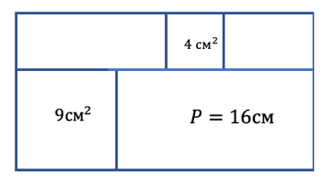
\includegraphics[scale=0.5]{kvadr.png}}
\end{figure}
\end{center}
Вася вырезал из бумаги два квадрата и три прямоугольника, а затем сложил из них большой прямоугольник (см. рисунок). Найдите площадь  полученного Васей прямоугольника, если площади квадратов равны $4\text{ см}^2$ и $9\text{ см}^2,$ а периметр одного из прямоугольников --- 16 см.\\
250. За какое время при движении против течения реки теплоход пройдёт 216 км, если его собственная скорость 15 км/ч, а скорость течения в 5 раз меньше собственной скорости теплохода?\\
251. За какое время при движении против течения реки теплоход пройдёт 204 км, если его собственная скорость 14 км/ч, а скорость течения в 7 раз меньше собственной скорости теплохода?\\
252. В некотором году в мае было пятниц больше, чем суббот. А какого числа в том году был второй вторник сентября?\\
253. В некотором году в мае было четвергов больше, чем пятниц. А какого числа в том году был второй вторник сентября?\\
254. В домике на шоссе живёт велосипедист Олег. Однажды он выехал из дома в магазин. Доехав до магазина, он сообразил, что забыл карточку, и поехал обратно в два раза быстрее. Он так сильно переживал, что проехал мимо своего дома некоторое расстояние. Повернув назад и ещё в два раза увеличив скорость, Олег успешно остановился у дома через 5 часов после того, как выехал из него. Сколько времени Олег ехал, удаляясь от своего дома? Ответ дайте в минутах.\\
255. В домике на шоссе живёт велосипедист Олег. Однажды он выехал из дома в магазин. Доехав до магазина, он сообразил, что забыл карточку, и поехал обратно в три раза быстрее. Он так сильно переживал, что проехал мимо своего дома некоторое расстояние. Повернув назад и ещё в три раза увеличив скорость, Олег успешно остановился у дома через 5 часов после того, как выехал из него. Сколько времени Олег ехал, приближаясь к своему дому? Ответ дайте в минутах.\\
256. Когда в Петербурге $12:12,$ то в Новосибирске $16:12.$ Когда в Новосибирске $12:15,$ то в Якутске $15:15.$ Самолёт вылетел из Якутска в Петербург в $13:15$ и летел 7 часов 40 минут. Во сколько он приземлился?\\
257. Когда в Петербурге $12:12,$ то в Екатеринбурге $14:12.$ Когда в Екатеринбурге $12:15,$ то в Хабаровске $17:15.$ Самолёт вылетел из Хабаровска в Петербург в $10:15$ и летел 8 часов 40 минут. Во сколько он приземлился?\\
258. Периметр прямоугольника равен 10 см. Чему равна площадь этого прямоугольника в квадратных сантиметрах, если его ширина равна 2 см?\\
259. Периметр прямоугольника равен 14 см. Чему равна площадь этого прямоугольника в квадратных сантиметрах, если его ширина равна 2 см?\\
260. Два пешехода одновременно вышли из магазина и пошли по прямой улице в противоположных направлениях. Скорость одного из них составляла 87 м/мин, скорость второго 98 м/мин. Какое расстояние будет между ними через 7 минут после выхода?\\
261. Два пешехода одновременно вышли из кафе и пошли по прямой улице в противоположных направлениях. Скорость одного из них составляла 76 м/мин, скорость второго 87 м/мин. Какое расстояние будет между ними через 9 минут после выхода?\\
262. Каток, имеющий форму прямоугольника, длина которого 57 м, а ширина 29 м, залит льдом, причём масса льда на одном квадратном метре катка составляет 10 кг. Найдите массу льда, покрывающего весь каток. Ответ выразите в килограммах.\\
263. Каток, имеющий форму прямоугольника, длина которого 47 м, а ширина 26 м, залит льдом, причём масса льда на одном квадратном метре катка составляет 10 кг. Найдите массу льда, покрывающего весь каток. Ответ выразите в килограммах.\\
264. На каждые 70 км пути машина расходует 6 л бензина. Сколько литров бензина потребуется, чтобы проехать 560 км?\\
265. На каждые 80 км пути машина расходует 7 л бензина. Сколько литров бензина потребуется, чтобы проехать 560 км?\\
266. Сколько квадратных дециметров в $800\text{ см}^2?$\\
267. Сколько квадратных дециметров в $600\text{ см}^2?$\\
268. 200 г конфет стоят 58 рублей. Сколько стоят 300 г таких конфет?\\
269. 300 г орехов стоят 87 рублей. Сколько стоят 200 г таких орехов?\\
270. На сколько секунд больше 5 минут 19 секунд, чем 3 минуты 48 секунд?\\
271. На сколько секунд больше 9 минут 23 секунды, чем 7 минут 57 секунд?\\
272. Птичка колибри во время полёта делает 1500 взмахов крыльями в минуту. Во время миграции колибри приходится лететь довольно далеко. Сколько взмахов крыльями делает колибри за полтора часа полёта?\\
273. Стрекоза во время полёта делает 1300 взмахов крыльями в минуту. Во время охоты стрекозе приходится много летать. Сколько взмахов крыльями делает стрекоза за полтора часа полёта?\\
274. Расстояние между двумя концами дорожки 32 м. Улитки ползут с разных концов дорожки навстречу друг другу. Скорость одной улитки 3 м/мин, скорость другой 4 м/мин. Каким будет расстояние между улитками через 7 минут, если они не будут останавливаться?\\
275. Расстояние между двумя концами дорожки 38 м. Две жужелицы ползут с разных концов дорожки навстречу друг другу. Скорость одной жужелицы 5 м/мин, скорость другой 4 м/мин. Каким будет расстояние между жужелицами через 6 минут, если они не будут останавливаться?\\
276. Нефтяной танкер привёз в порт 108000 галлонов нефти. Нефть из него выкачивают так, что за 2 часа объём нефти уменьшается на треть от того, который был в начале этих двух часов. Сколько галлонов нефти останется в танкере через 6 часов?\\
277. Молоковоз привёз на молокозавод 64000 пинт молока. Молоко из него сливают для переработки так, что за 3 часа объём молока уменьшается на четверть от того, который был в начале этих трёх часов. Сколько пинт молока останется в молоковозе через 9 часов?\\
278. Первая бегунья пробежала дистанцию 500 метров за 5 минут 10 секунд, а вторая бегунья пробежала дистанцию на 200 метров за 1 минуту 58 секунд. Если бы обе бегуньи бежали 400 метров каждая со своей скоростью, на сколько секунд вторая бегунья прибежала бы раньше, чем первая?\\
279. Первый бегун пробежал дистанцию 200 метров за 1 минуту 56 секунд, а второй бегун пробежал дистанцию 700 метров за 7 минут и 21 секунду. Если бы оба бегуна бежали 400 метров каждый со своей скоростью, на сколько секунд первый бегун прибежал бы раньше второго?\\
280. Два тигра за 4 часа могут съесть одну печеньку. Сколько тигров нужно, чтобы за 1 час съесть три печеньки?\\
281. Два тигра за 8 часов могут съесть одну печеньку. Сколько тигров нужно, чтобы за 1 час съесть две печеньки?\\
282. В течение 2021 года Катя покупала по одной конфете каждую субботу и каждый вторник, а в другие дни недели Катя не покупала конфет. Сколько конфет в 2021 году купила Катя, если 1 января 2021 года была пятница?\\
283. В течение 2021 года Катя покупала по одной конфете каждую пятницу и каждую среду, а в другие дни недели Катя не покупала конфет. Сколько конфет в 2021 году купила Катя, если 1 января 2021 года была пятница?\\
284. На первом складе было 480 кг конфет, а на втором --- в 3 раза больше. Все конфеты разложили в коробки по 12 кг в каждую. Одну четвёртую часть всех конфет отправили в магазин, а одну шестую часть остатка --- в детские сады. Сколько коробок с конфетами отправили в детские сады? Сколько коробок осталось?\\
285. Хоттабыч ехал на ослике 24 минуты, а потом летел на ковре-самолёте путь вдвое больший. Сколько времени он летел, если скорость ковра-самолёта в шесть раз больше, чем у ослика?\\
286. Если в Петербурге $12:12,$ то в Калининграде $11:12.$ Когда в Новосибирске $03:15,$ в Калининграде $22:15.$ Самолёт вылетел из Новосибирска в Москву в $13:20$ и летел 4 часа 40 минут. Во сколько он приземлился?\\
287. Если в Петербурге $12:12,$ то в Калининграде $11:12.$ Когда в Иркутске $04:15,$ в Калининграде $22:15.$ Самолёт вылетел из Иркутска в Москву в $10:20$ и летел 5 часов 40 минут. Во сколько он приземлился?\\
288. Вступительная олимпиада в 5 класс проводится в предпоследнее воскресенье мая. Каким по счёту днём года может быть день вступительной работы? Например, 1 февраля --- 32-й день года. Перечислите все возможные варианты.\\
289. Показ работ вступительной олимпиады в 5 класс проводится в предпоследний вторник мая. Каким по счёту днём года может быть день показа работ? Например, 1 февраля --- 32-й день года. Перечислите все возможные варианты.\\
290. На прямой дороге расположены три домика. Из них одновременно вышли три человека. Первый пошёл направо со скоростью 4 километра в час, а второй и третий --- налево со скоростью 3 и 5 километров в час соответственно. Первый встретил второго через 3 часа, а третьего --- через 3 часа 40 минут после выхода. Через какое время после встречи с первым третий догонит второго?\\
291. На прямой дороге расположены три домика. Из них одновременно вышли три человека. Первый пошёл направо со скоростью 3 километра в час, а второй и третий --- налево со скоростью 4 и 5 километров в час соответственно. Первый встретил второго через 3 часа, а третьего --- через 3 часа 15 минут после выхода. Через какое время после встречи с первым третий догонит второго?\\
292. Периметр прямоугольника равен 36 см. Если провести некоторый вертикальный разрез, то сумма периметров двух полученных прямоугольников будет равна 45 см. А чему будет равен периметр каждого из прямоугольников, если горизонтальным разрезом поделить исходный прямоугольник на два равных?\\
293. Периметр прямоугольника равен 38 см. Если провести некоторый вертикальный разрез, то сумма периметров двух полученных прямоугольников будет равна 45 см. А чему будет равен периметр каждого из прямоугольников, если горизонтальным разрезом поделить исходный прямоугольник на два равных?\\
294. Петя взял деревянный куб со стороной 60 см и распилил его на бруски размером $1\cdot2\cdot3$ дециметра. А Коля распилил такой же куб на бруски размером $6\times6\times12$см. У кого получилось больше брусков и на сколько?\\
295. Коля взял деревянный куб со стороной 60 см и распилил его на бруски размером $1\cdot2\cdot3$ дециметра. А Петя распилил такой же куб на бруски размером $6\times5\times10$см. У кого получилось больше брусков и на сколько?\\
296. Васины часы уходят вперёд на 15 минут в день, а часы Пети отстают на 10 минут в день. 1 мая в полдень на Васиных часах $17:00,$ а на Петиных $13:00.$ Какого числа и какого месяца впервые после 1 мая в полдень их часы покажут одинаковое время одновременно?\\
297. Васины часы уходят вперёд на 10 минут в день, а часы Пети отстают на 15 минут в день. 10 мая в полдень на Васиных часах $19:00,$ а на Петиных $15:00.$ Какого числа и какого месяца впервые после 10 мая в полдень их часы покажут одинаковое время одновременно?\\
298. Какой день недели будет через 10 дней, если послезавтра будет вторник?\\
299. Какой день недели будет через 10 дней, если позавчера была пятница?\\
300. Машина проезжает 18 метров за секунду. А сколько дециметров проедет машина за минуту?\\
301. Машина проезжает 17 метров за секунду. А сколько дециметров проедет машина за минуту?\\
302. Есть труба, в левый конец которой поступает вода со скоростью 1 литр за 35 секунд. Посередине трубы есть небольшая течь, поэтому вода вытекает из правого конца трубы со скоростью 1 литр за 36 секунд. Под место протекания поставили пустую литровую банку. За сколько минут наполнится банка?\\
303. Есть труба, в левый конец которой поступает вода со скоростью 1 литр за 44 секунд. Посередине трубы есть небольшая течь, поэтому вода вытекает из правого конца трубы со скоростью 1 литр за 45 секунд. Под место протекания поставили пустую литровую банку. За сколько минут наполнится банка?\\
304. Маша может добраться до школы за 38 минут, пройдя 25 минут пешком и проехав 13 минут на скейтборде. Также Маша может добраться до школы за 31 минуту, пройдя 11 минут пешком и проехав 20 минут на скейтборде. А сколько минут потребуется Маше, чтобы пройти весь путь до школы пешком?\\
305. Маша может добраться до школы за 40 минут, пройдя 26 минут пешком и проехав 14 минут на скейтборде. Также Маша может добраться до школы за 32 минуты, пройдя 10 минут пешком и проехав 22 минуты на скейтборде. А сколько минут потребуется Маше, чтобы пройти весь путь до школы пешком?\\
306. Поезд проехал 360 км за 5 часов с постоянной скоростью, после чего увеличил скорость на 9 км/ч и ехал ещё 3 часа. Сколько всего километров проехал поезд?\\
307. На одной дороге расположены город, посёлок и деревня (в таком порядке). Расстояние между посёлком и городом 20 км. Из города в деревню выезжает автобус, а через минуту после его старта из посёлка в деревню выезжает грузовик со скоростью 60 км/ч. Каждые 10 км автобус делает остановку на 1 минуту, а грузовик едет без остановок. Автобус догоняет грузовик через 1 час 40 минут после старта грузовика и в этот момент снова делает остановку на 1 минуту. Грузовик же продолжает ехать вперёд. Через какое время автобус во второй раз догонит грузовик? Каково расстояние от города до деревни, если от момента первой встречи грузовика и автобуса до прибытия автобуса в деревню прошло 34 минуты?\\
308. Дешёвая батарейка стоит в три раза дешевле дорогой. При этом в фонарике дешёвая батарейка работает 2 часа 37 минут, а дорогая работает 8 часов. Что прослужит дольше и на сколько минут --- три дешёвых батарейки или одна дорогая?\\
309. Дешёвая ручка стоит в четыре раза дешевле дорогой. При этом ей можно непрерывно писать 1 час 23 минуты, а дорогой ручкой можно писать 5 часов 30 минут. Что прослужит дольше и на сколько минут --- четыре дешёвых ручки или одна дорогая?\\
310. Периметр квадрата равен 32 см и составляет четверть периметра прямоугольника. Найдите площадь прямоугольника, если его ширина на 6 см меньше длины.\\
311. Периметр квадрата равен 54 см и составляет треть периметра прямоугольника. Найдите площадь прямоугольника, если его ширина на 9 см меньше длины.\\
312. Олег наполняет водой бассейн, имеющий форму параллелепипеда высотой 1 м, ширина и длина которого по 2 м. В одно ведро помещается $16\text{ дм}^3$ воды. Олег уже вылил в бассейн 40 вёдер. Какова глубина наполненной части бассейна? Выразите ответ в сантиметрах.\\
313. Лёша наполняет водой бассейн, имеющий форму параллелепипеда высотой 1 м, ширина и длина которого по 3 м. В одно ведро помещается $12\text{ дм}^3$ воды. Лёша уже вылил в бассейн 90 вёдер. Какова глубина наполненной части бассейна? Выразите ответ в сантиметрах.\\
314. Автобус движется между двумя городами с постоянной скоростью. Через 5 часов после начала движения ему остаётся проехать 450 км, а через 7 часов после начала движения остаётся 280 км. Найдите расстояние между городами.\\
315. Автобус движется между двумя городами с постоянной скоростью. Через 4 часа после начала движения ему остаётся проехать 385 км, а через 6 часов после начала движения остаётся 215 км. Найдите расстояние между городами.\\
316. На отрезке $AB$ отмечены точки $C$ и $K$ в таком порядке. Точка $E$ --- середина $AC,$ точка $P$ --- середина $KB.\ AB = 80$см; сумма $AE$ и $PB$ равна 19 см. Найдите длину $CK.$\\
317. На отрезке $MK$ отмечены точки $A$ и $B$ в таком порядке. Точка $O$ --- середина $AM,$ точка $C$ --- середина $KB.\ AB = 70$см; сумма $AO$ и $CB$ равна 14 см. Найдите длину $MK.$\\
318. Когда в городе Бубуду 1 час 32 минуты, в городе Дудубу 23 часа 32 минуты. Самолёт вылетает из Бубуду в 13 часов 45 минут по местному времени и приземляется в
Дудубу в 15 часов 20 минут по местному времени. Сколько длится полёт?\\
319. Когда в городе Тотомо 2 часа 13 минут, в городе Момото 23 часа 13 минут. Самолёт вылетает из Момото в 15 ч 20 мин по местному времени и приземляется в Тотомо в
23 ч 35 минут по местному времени. Сколько длится полёт?\\
320. Из прямоугольника со сторонами 12 см и 19 см вырезали прямоугольник со сторонами 7 см и 12 см. Оставшуюся часть разрезали на квадраты со стороной 1 см. Из всех них удалось сложить квадрат. Чему равна его площадь? Чему равна длина его стороны?\\
321. Из прямоугольника со сторонами 14 см и 22 см вырезали прямоугольник со сторонами
7 см и 16 см. Оставшуюся часть разрезали на квадраты со стороной 1 см. Из всех них удалось сложить квадрат. Чему равна его площадь? Чему равна длина его стороны?\\
322. Строительной бригаде надо огородить прямоугольный участок площадью $40\text{ м}^2.$ Для постройки забора они используют секции длиной 2 м. Каким может быть
наименьший периметр такого участка? Секции можно скреплять только концами. Ответ дайте в метрах.\\
323. Строительной бригаде надо огородить прямоугольный участок площадью $54\text{ м}^2.$ Для постройки забора они используют секции длиной 3 м. Каким может быть
наибольший периметр такого участка? Секции можно скреплять только концами. Ответ дайте в метрах.\\
324. Во сколько раз автомобиль, который едет со скоростью 60 км/ч, быстрее велосипедиста, едущего со скоростью 200 м/мин?\\
325. Во сколько раз автомобиль, который едет со скоростью 90 км/ч, быстрее велосипедиста, едущего со скоростью 300 м/мин?\\
326. Строители кладут плитку на пол в квадратной комнате. Сторона комнаты равна целому числу метров. Строители использовали 16 плиток 2 на 2 метра,
но некоторые не целиком. Какая могла быть максимальная площадь комнаты?\\
327. Строители кладут плитку на пол в квадратной комнате. Сторона комнаты равна целому числу метров. Строители использовали 9 плиток 2 на 2 метра,
но некоторые не целиком. Какая могла быть максимальная площадь комнаты?\\
328. Машина едет по длинному проспекту, на котором установлено 29 светофоров. Проспект начинается и заканчивается светофором. Светофоры зажигаются одновременно и горят зелёным 3 минуты для пешеходов, а затем 2 минуты 30 секунд для машин. Расстояние между соседними
светофорами автомобилист всегда проезжает за 1 минуту. Сколько времени понадобится машине, чтобы проехать весь проспект целиком? Машина начинает движение по проспекту сразу, как только загорается зелёный свет на первом светофоре.\\
329. Машина едет по длинному проспекту, на котором установлен 31 светофор. Проспект начинается и заканчивается светофором. Светофоры зажигаются одновременно и горят зелёным 2 минуты для пешеходов, а затем 3 минуты 30 секунд для машин. Расстояние между соседними светофорами автомобилист всегда проезжает за 1 минуту. Сколько времени понадобится машине, чтобы проехать весь проспект целиком? Машина начинает движение по проспекту сразу, как только загорается зелёный свет на первом светофоре.\\
330. Дан прямоугольник, длины сторон которого выражаются целым числом сантиметров. Оказалось, что можно отрезать от него прямоугольник периметра 420 см, и получится квадрат. Также оказалось, что можно приклеить к нему прямоугольник периметра 660 см, и получится квадрат. Придумайте такой прямоугольник, в ответ запишите обе его стороны.\\
331. Дан прямоугольник, длины сторон которого выражаются целым числом сантиметров. Оказалось, что можно отрезать от него прямоугольник периметра 420 см, и получится квадрат. Также оказалось, что можно приклеить к нему прямоугольник периметра 600 см, и получится квадрат. Придумайте такой прямоугольник, в ответ запишите обе его стороны.\\
332. В мае некоторого года суббот было больше, чем четвергов. Каким днём недели могло быть 30 января того года?\\
333. В мае некоторого года пятниц было больше, чем сред. Каким днём недели могло быть 30 января того года?\\
334. По круглому стадионе на самокате ездит тренер со скоростью 12 км/ч. Навстречу ему передвигается Максим с постоянной скоростью. Тренер заметил, что они постоянно встречаются в 4 разных точках этого круга. Чему может быть равна скорость Максима?\\
335. По круглому стадионе на самокате ездит тренер со скоростью 15 км/ч. Навстречу ему передвигается Максим с постоянной скоростью. Тренер заметил, что они постоянно встречаются в 4 разных точках этого круга. Чему может быть равна скорость Максима?\\
336. Параллелепипед $4\times4\times5$ облили краской и распилили на кубики со стороной 1. У скольких из полученных кубиков число окрашенных граней чётное?\\
337. Параллелепипед $4\times5\times5$ облили краской и распилили на кубики со стороной 1. У скольких из полученных кубиков число окрашенных граней чётное?\\
338. Сегодня 19 мая 2024 года. Какой будет месяц через 300 дней?\\
339. Сегодня 19 мая 2024 года. Какой будет месяц через 330 дней?\\
340. Когда в Брянске 10:17, в Хабаровске 17:17. Когда в Хабаровске 15:12, в Кургане 10:12. Путешественник выехал из Кургана в 12:01 и приехал на следующий день в Брянск в 03:46 местного времени. Сколько времени он путешествовал?\\
341. Когда в Брянске 10:17, в Хабаровске 17:17. Когда в Хабаровске 15:12, в Кургане 10:12. Путешественник выехал из Брянска в 13:23 и приехал на следующий день в Курган в 05:45 местного времени. Сколько времени он путешествовал?
\newpage
